\documentclass[aspectratio=169,11pt]{beamer}

\usetheme{Madrid}
\usecolortheme{crane}
\setbeamertemplate{navigation symbols}{}

% Personnalisation rouge
\definecolor{darkred}{RGB}{139,0,0}
\definecolor{brightred}{RGB}{220,20,60}
\definecolor{lightred}{RGB}{255,192,203}
\setbeamercolor{title}{fg=white,bg=darkred}
\setbeamercolor{frametitle}{fg=white,bg=darkred}
\setbeamercolor{section in head/foot}{bg=brightred,fg=white}
\setbeamercolor{alerted text}{fg=darkred}

\usepackage[T1]{fontenc}
\usepackage[utf8]{inputenc}
\usepackage[french]{babel}
\usepackage{graphicx}
\usepackage{booktabs}
\usepackage{amsmath}
\usepackage{hyperref}

\graphicspath{{figures_feu/}}

\title{Dynamique du feu en foret boreale}
\subtitle{Analyse regionale 12\,000 ans et variabilite par lac}
\author{Reconstruction paleofeu -- Analyse exploratoire}
\institute{Foret Boreale}
\date{\today}

\begin{document}

\begin{frame}
  \titlepage
\end{frame}

\begin{frame}{Plan de presentation}
  \tableofcontents
\end{frame}

\section{1. Contexte et objectifs}

\begin{frame}{Motivations scientifiques}
\begin{itemize}
  \item \alert{Question centrale}: Comment evolue le regime du feu boreale sur les 12 derniers millenaires?
  
  \item \alert{Enjeu:} Distinguer signal regional robuste vs heterogeneite locale (specificite par site).
  
  \item \alert{Approche:} Multi-echelle spatiale + temporelle detaillee.
  \begin{itemize}
    \item Proxies regionaux lissés (tendances).
    \item Chronologies par lac (variabilite fine).
  \end{itemize}
\end{itemize}
\end{frame}

\begin{frame}{Donnees et metriques}
\textbf{3 indicateurs paleofeu regionaux (lissage centre w=101):}
\begin{itemize}
  \item \alert{RegBB}: biomasse brulee lissee (mm² cm$^{-1}$ yr$^{-1}$).
  \item \alert{RegFRI}: intervalle de retour = 1 / frequence feu (ans).
  \item \alert{RegFS}: indice taille-severite (adimensionnel).
\end{itemize}

\textbf{6 lacs archeopalynologiques:} M14, M15, O6, O14, O15, O16.

\textbf{Perimetre temporel:} 0--12\,000 cal. yr BP. IC 90\% sur tous les indicateurs.

\textbf{Source donnees:} Bootstrap charbon + Lake\_fire\_frequency (evenements discrets).
\end{frame}

\section{2. Resultats regionaux}

\begin{frame}{Figure 2: Regimes regionaux 12\,000 ans}
  \centering
  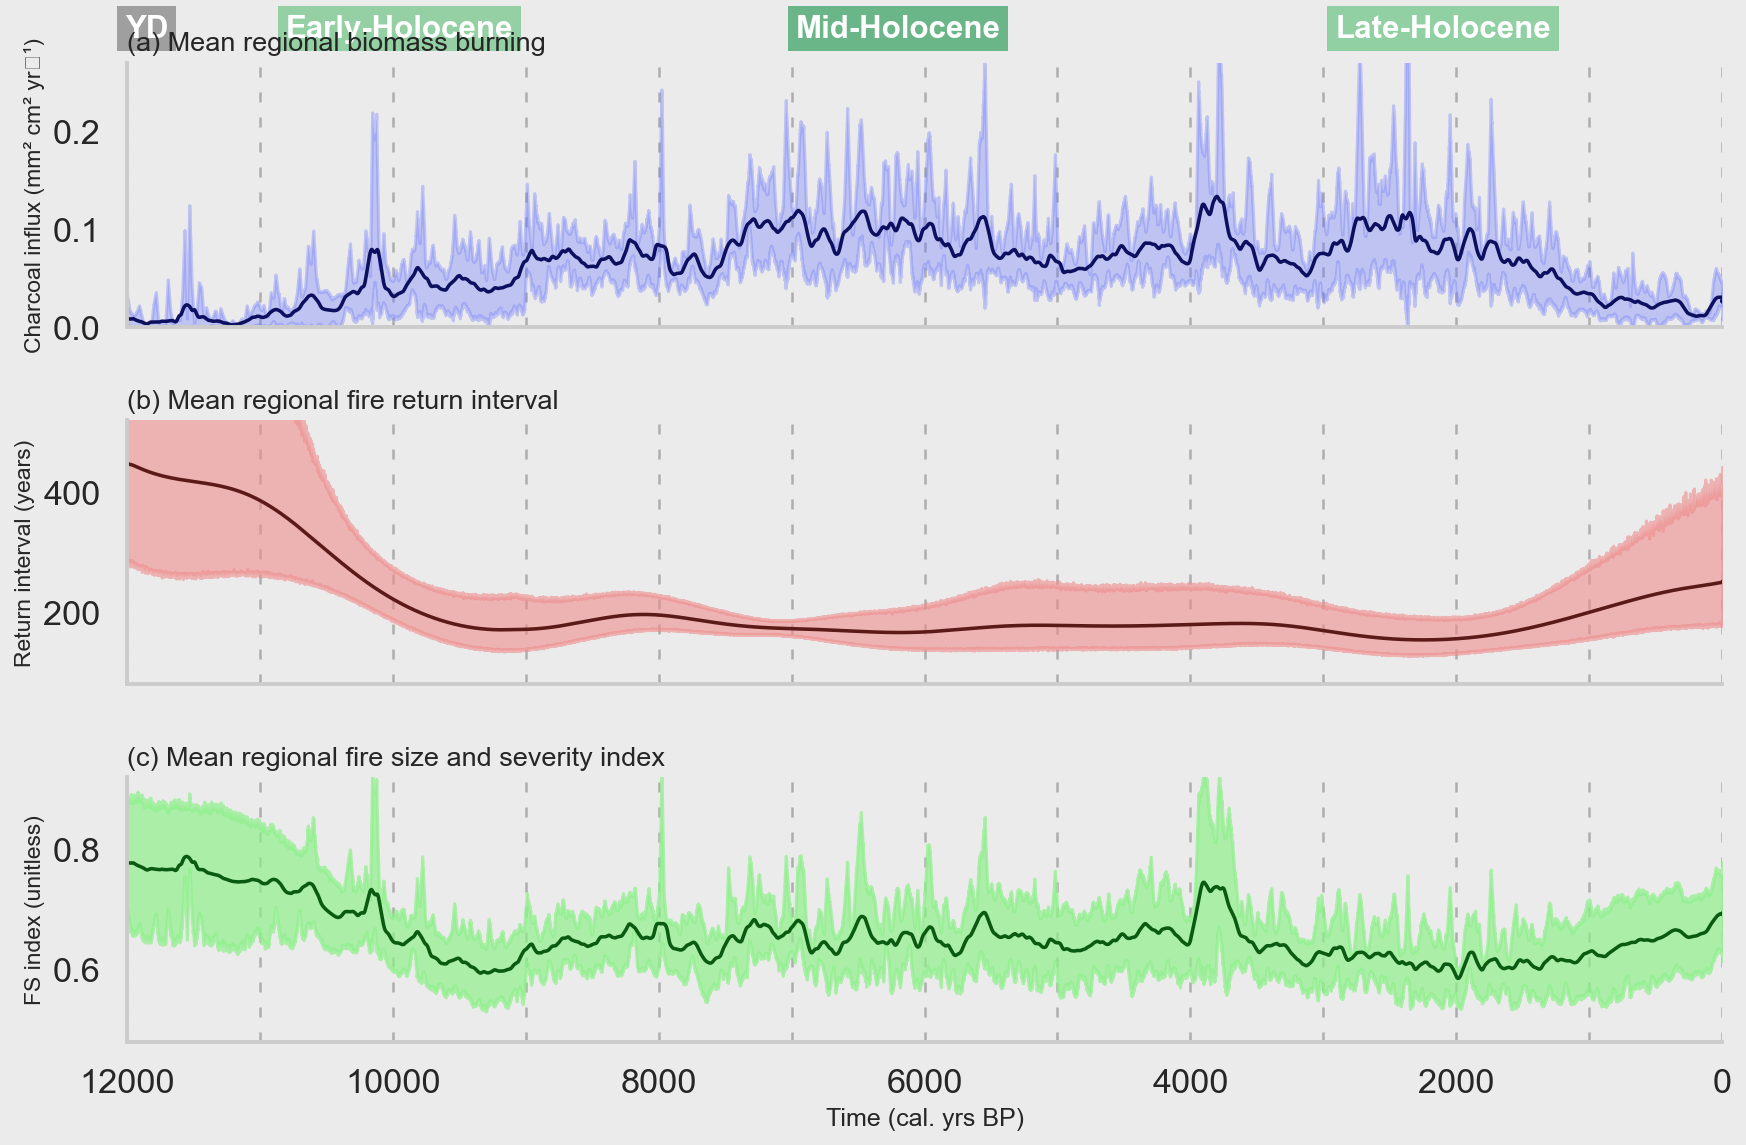
\includegraphics[width=0.7\linewidth]{fig_02_regional_fire_history.png}
\end{frame}

\begin{frame}{Lecture detaillee panneau (a) -- RegBB (biomasse brulee)}
\small
\begin{itemize}
  \item \alert{~12--11 ka}: Valeur minimale, $\approx 0.00$--0.02 mm² cm$^{-1}$ yr$^{-1}$. Transition Pleistocene/Holocene.
  
  \item \alert{~10--8 ka}: Montee progressive, debut du plateau.
  
  \item \alert{\textbf{~8--2 ka (PLATEAU ELEVE)}}: RegBB se stabilise \textbf{0.06--0.12}. 
  \begin{itemize}
    \item Pics absolus: $\approx 0.10$--0.12 autour de 7--6 ka et 4 ka.
    \item Minimum partiel (~0.05) vers 9 ka.
  \end{itemize}
  
  \item \alert{~2--0 ka}: Baisse nette a 0.02--0.04. Tendance a l'apaisement.
  
  \item IC 90\% s'elargit notablement aux extremites (< 2 ka et > 10 ka).
\end{itemize}
\textbf{Interpretation:} Holocene moyen = zone d'activite combustion maximale. Stabilite externe bien documentee.
\end{frame}

\begin{frame}{Lecture detaillee panneau (b) -- RegFRI (intervalle de retour)}
\small
\begin{itemize}
  \item \alert{~12 ka}: FRI $\approx 430$--450 ans. Feux \textbf{tres espaces}.
  
  \item \alert{~10--8 ka}: Baisse progressive, FRI vers 300--250 ans.
  
  \item \alert{\textbf{~8--4 ka (MINIMUM)}}: FRI chute a \textbf{170--200 ans}. Feux rapproches, intense.
  \begin{itemize}
    \item Minimum absolu: ~150 ans vers 6 ka.
  \end{itemize}
  
  \item \alert{~4--2 ka}: Remontee lente, FRI $\approx$ 200--250 ans.
  
  \item \alert{~2--0 ka}: Stabilisation a \textbf{250+ ans}. Return a regime moins actif.
\end{itemize}
\textbf{Interpretation:} La frequence de feu est le parametre le plus discriminant Holocene-wide. Haut contraste debut/milieu.
\end{frame}

\begin{frame}{Lecture detaillee panneau (c) -- RegFS (taille/severite)}
\small
\begin{itemize}
  \item \alert{~12--10 ka}: RegFS eleve, ~0.77--0.79. Feux plutot importants individuellement.
  
  \item \alert{~9 ka}: Creux marque (~0.60). Transition temporelle.
  
  \item \alert{~8--5 ka}: Remontee progressive a ~0.68--0.72.
  
  \item \alert{\textbf{~4 ka (PIC)}}: RegFS atteint ~0.76--0.77. Feux de grande taille.
  
  \item \alert{~3--0 ka}: Variabilite mais tendance a la baisse final.
\end{itemize}
\textbf{Interpretation:} Severite correlée (mais non biunivoque) avec RegBB et FRI. Pic de 4 ka majeur.
\end{frame}

\begin{frame}[fragile]{Synthese regionale: 3 phases distinctes}
\centering
\small
\begin{tabular}{|c|c|c|c|c|}
\hline
\textbf{Phase} & \textbf{Periode} & \textbf{RegBB} & \textbf{RegFRI} & \textbf{Regime} \\
\hline
Debut & 12--10 ka & Faible & Eleve (400++) & Feux \textit{rares}, severes \\
\hline
\alert{OPTIMUM} & \textbf{8--4 ka} & \textbf{Soutenu} & \textbf{Bas} & \textit{Frequents}, intensos \\
\hline
Recent & 2--0 ka & Baisse & Hausse & Feux moins actifs \\
\hline
\end{tabular}

\vspace{0.5cm}
\textbf{Message majeur:} Non-linearite evidente. L'Holocene moyen (4--8 ka) n'est \alert{PAS} une extrapolation des extre\-mites. Seuil d'activite clairement identifie.
\end{frame}

\begin{frame}{Zoom 4000--6000 cal BP (exemple detaille)}
  \centering
  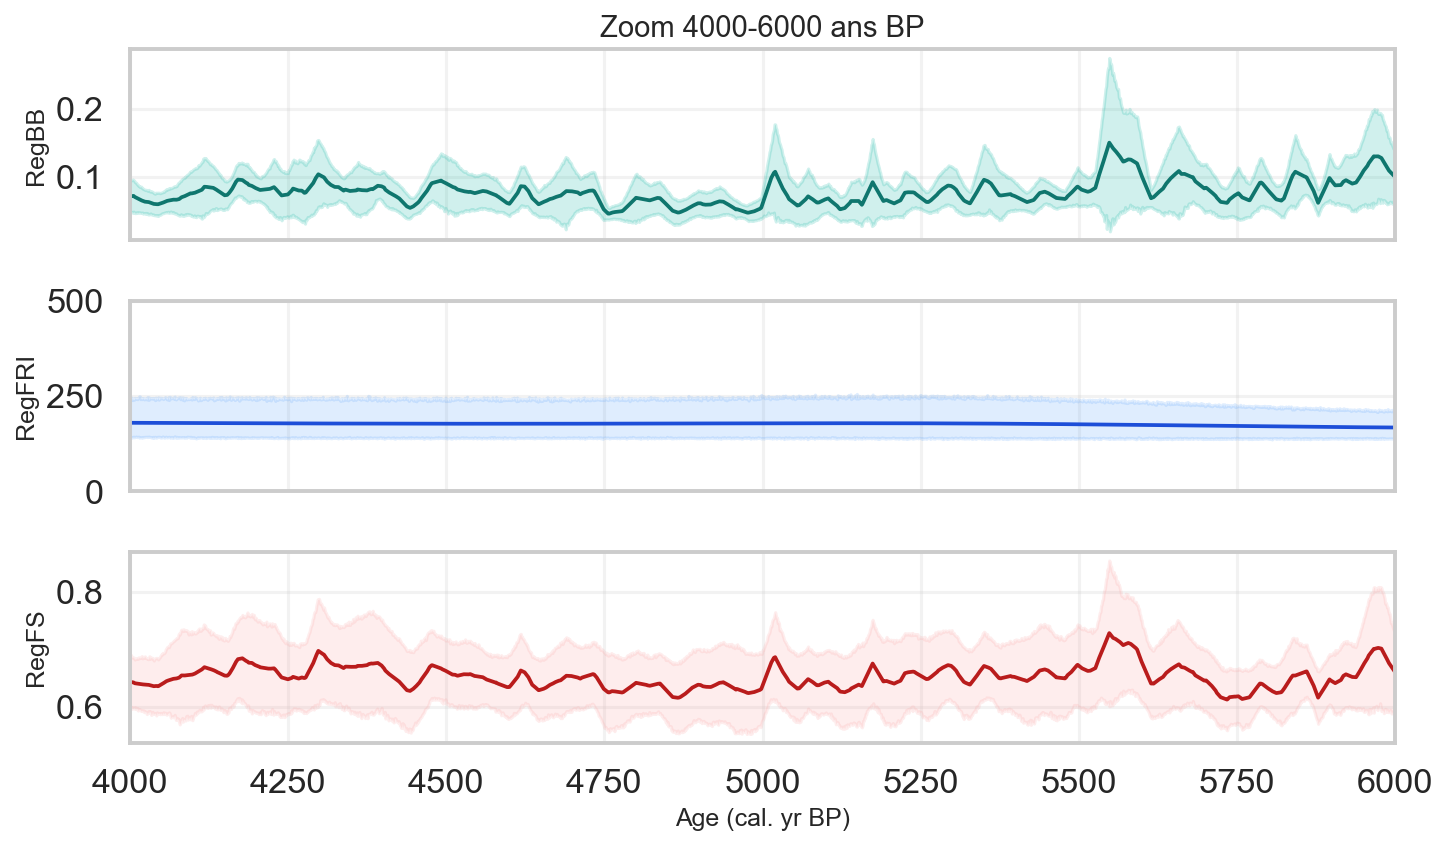
\includegraphics[width=0.5\linewidth]{fig_05_zoom_4000_6000_bp.png}
\end{frame}

\begin{frame}{Synthese zooms 2000 ans (7 fenetres)}
\small
\begin{itemize}
  \item \alert{10--12 ka}: Transition abrupte. FRI maximum, RegBB minimum.
  
  \item \alert{8--10 ka}: Decroissance FRI, RegBB monte progressivement. Transition vers optimum.
  
  \item \alert{\textbf{6--8 ka}}: Plateau maximal. RegBB $\approx 0.08$--0.10, FRI $\approx 150$--170 ans. ZONE REFERENCE.
  
  \item \alert{\textbf{4--6 ka}}: Maintien du plateau avec variabilite interne (pic ~4 ka). Robustesse du signal.
  
  \item \alert{2--4 ka}: Variabilite croissante, tendance decroissante amorcee.
  
  \item \alert{0--2 ka}: Baisse confirmee (RegBB $\downarrow$, FRI $\uparrow$). Transition vers regime recent.
\end{itemize}

\textbf{Conclusion:} Fenetre 4--8 ka concentre la majorite du signal paleo-feu haute-intensite = \alert{OPTIMUM DEFINITIF}.
\end{frame}

\section{3. Variabilite inter-lacs}

\begin{frame}{Comptage par lac: hierarchie d'influence}
  \centering
  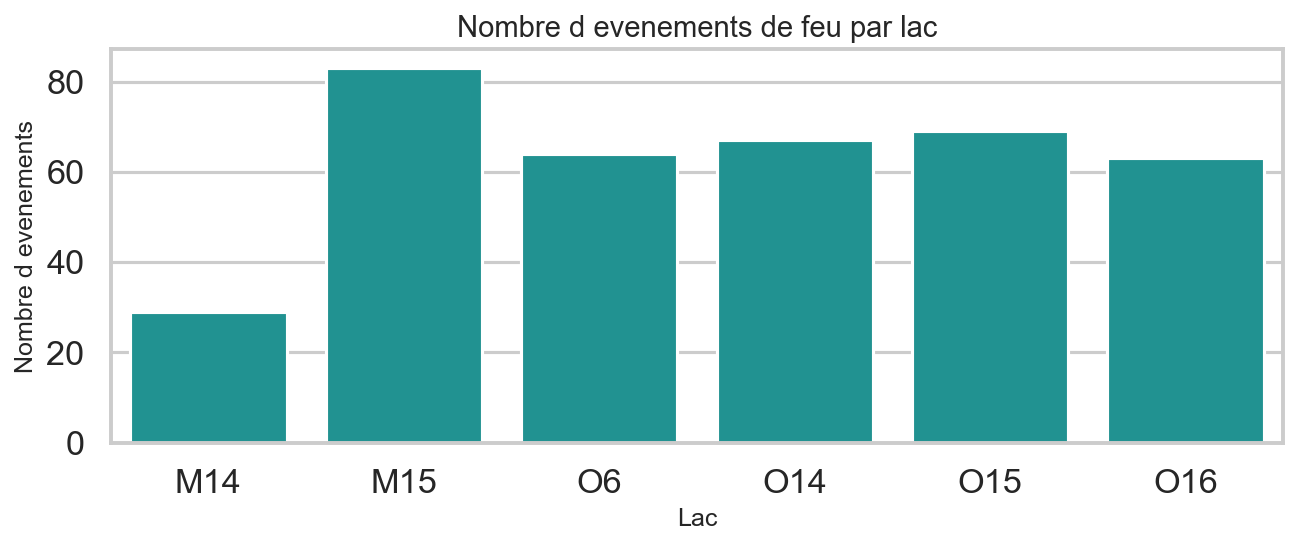
\includegraphics[width=0.75\linewidth]{fig_02_evenements_par_lac.png}
\end{frame}

\begin{frame}[fragile]{Rangs et contributions relatives}
\small
\centering
\begin{tabular}{|l|c|c|c|}
\hline
\textbf{Lac} & \textbf{Evenements} & \textbf{Pourcentage} & \textbf{Role} \\
\hline
M15 & 83 & 28\% & \alert{DOMINANT} \\
\hline
O15 & 67 & 22\% & Principal \\
\hline
O14 & 67 & 22\% & Principal \\
\hline
O16 & 68 & 23\% & Principal \\
\hline
O6 & 63 & 21\% & Secondaire \\
\hline
M14 & 29 & 10\% & Marginal \\
\hline
\textbf{Total} & \textbf{297} & 100\% & \\
\hline
\end{tabular}

\vspace{0.4cm}
\textbf{Observations clefs:}
\begin{itemize}
  \item M15 pilote ~28\%. Tres influent mais \alert{ne domine pas seul}.
  \item 5 lacs (sauf M14) contribuent ~27\% chacun moyenne $\approx$ balance regionale robuste.
  \item M14 marginal (~10\%) mais presence confirmee.
\end{itemize}
\end{frame}

\begin{frame}{Distribution des ages: densite spatio-temporelle}
  \centering
  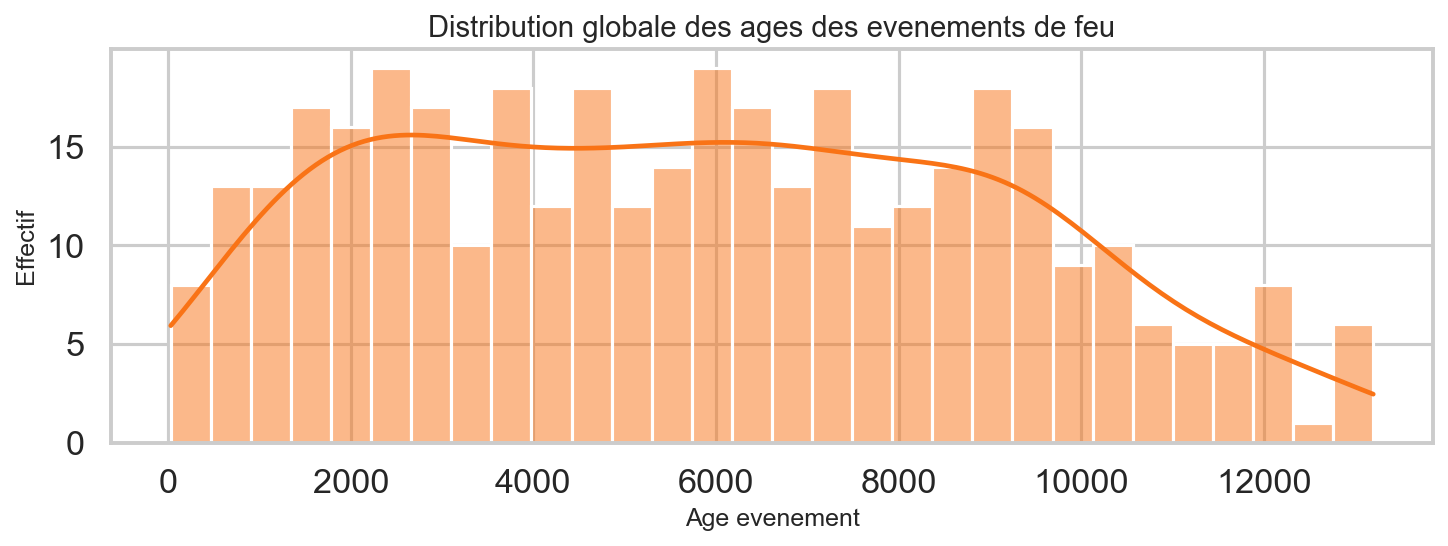
\includegraphics[width=0.8\linewidth]{fig_03_distribution_ages_evenements.png}
\end{frame}

\begin{frame}{Message distribution: ou se concentre l'activite?}
\begin{itemize}
  \item \alert{~85\% des 297 evenements}: fenetre 1500--10000 cal BP.
  
  \item \alert{Extremement rare} avant 11 ka et apres 500 cal BP.
  
  \item Distribution unimodale avec mode ~5000 cal BP (pic central).
  
  \item Asymetrie: queue plus longue vers ages recents (remanies?).
\end{itemize}

\textbf{Synthese:} Activite paleofeu regionale temporellement concentree = \alert{fausse pre-MHHG (climat optimum), vraie APRES 10 ka = coherence climate-feu}.
\end{frame}

\begin{frame}{Heatmap 1000 ans: pics locaux par periode}
  \centering
  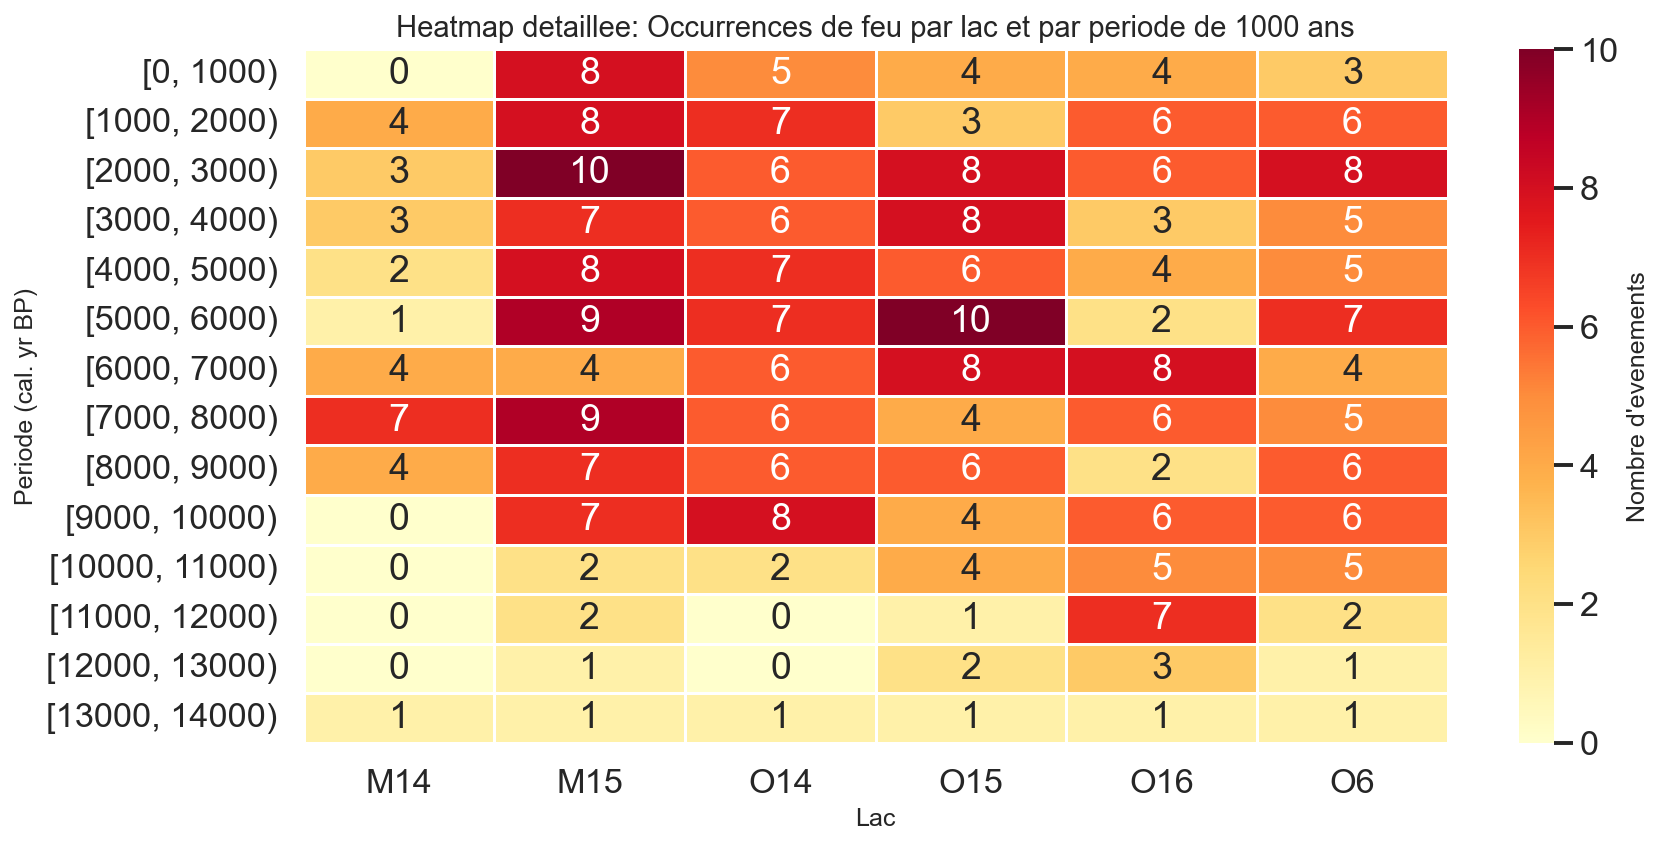
\includegraphics[width=0.7\linewidth]{fig_05_heatmap_occurrences_par_lac_1000ans.png}
\end{frame}

\begin{frame}{Lecture heatmap (binning 1000 ans)}
\small
\textbf{Pics absolus observes:}
\begin{itemize}
  \item M15 @ 2--3 ka: \alert{10 evenements}. Maximum global pour ce lac, synchrone pic RegBB regional.
  
  \item O15 @ 5--6 ka: \alert{10 evenements}. Aligne optimum moyen Holocene.
  
  \item O16 @ 6--7 ka et 9--10 ka: max ~8 ev./tranche. Double pic temporel.
\end{itemize}

\textbf{Competiteurs reguliers:}
\begin{itemize}
  \item O14: profil quasi-uniforme 1--10 ka (~6--8 ev./tranche). Fiabilite elevee.
  
  \item O6: lisse, 5--7 ev./tranche. Distribution reguliere.
\end{itemize}

\textbf{Heterogeneite markante:}
\begin{itemize}
  \item M14: dominance evidents avant 9 ka, puis quasi-zero apres. Desynchronisation locale.
  
  \item O16: activite double-pic (6--7 ka et 9--10 ka) contraste mono-pic autres lacs.
\end{itemize}
\end{frame}

\begin{frame}{Chronogramme 1000 ans (stacked timeline)}
  \centering
  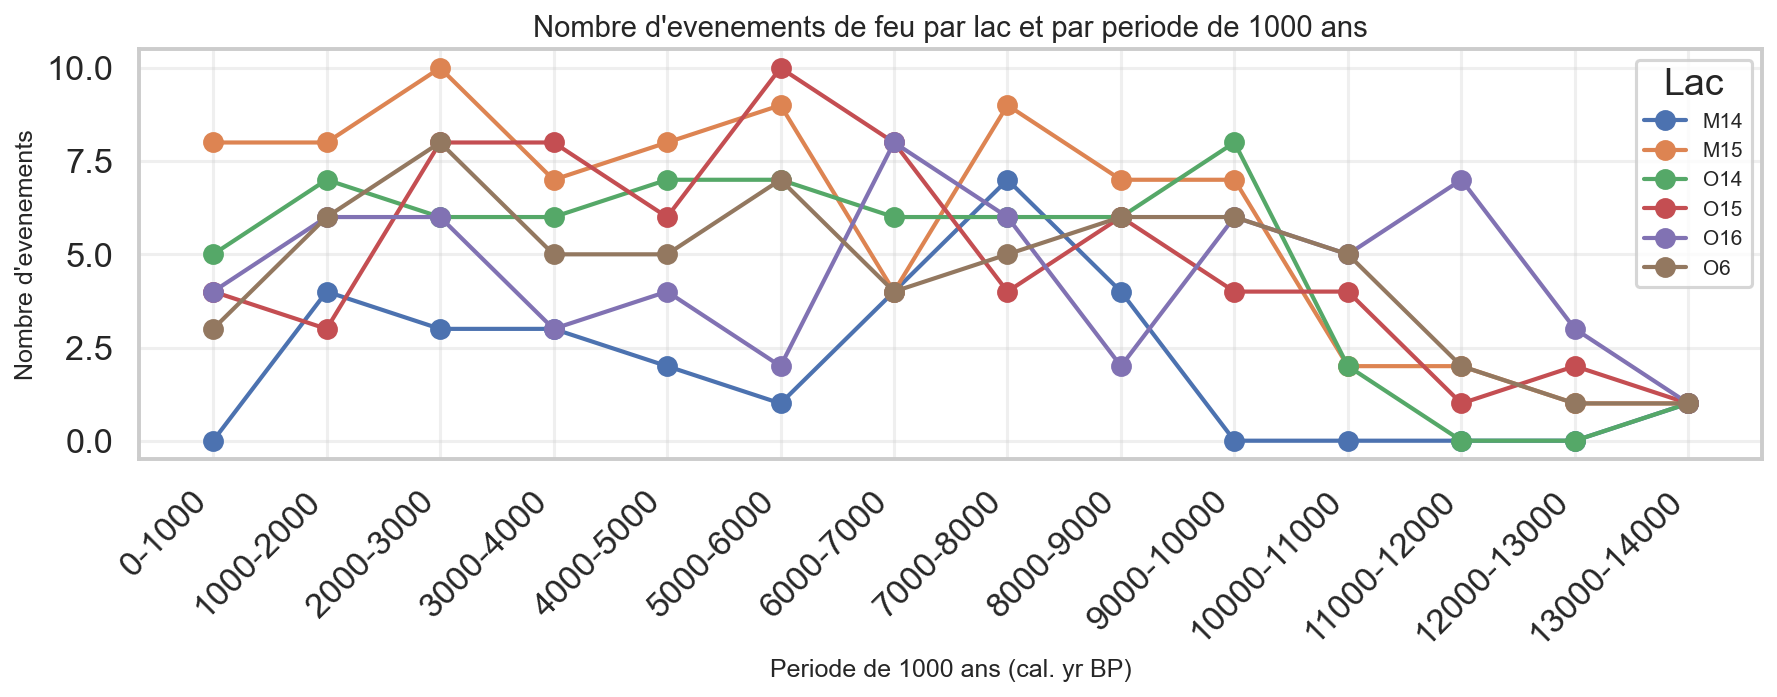
\includegraphics[width=0.85\linewidth]{fig_06_timeline_occurrences_par_lac_1000ans.png}
\end{frame}

\begin{frame}{Points saillants synchronite/asynchronite}
\begin{itemize}
  \item \alert{Forte convergence inter-lacs}: 2--9 ka (presque tous lacs maximaux ensemble dans memes fenetres).
  
  \item \alert{Domaines desynchronises}:
  \begin{itemize}
    \item O16 declination apres 5 ka (sorties du regime regional).
    \item M14 rarete apres 9 ka (possibles limites taphonomiques).
  \end{itemize}
  
  \item \alert{Robustesse globale}: Malgre desynchronisations, signal regional persiste = \textbf{fiable}.
\end{itemize}
\end{frame}

\section{4. Chronologies lac par lac}

\begin{frame}{Lac M15 (dominant, 83 evenements)}
  \centering
  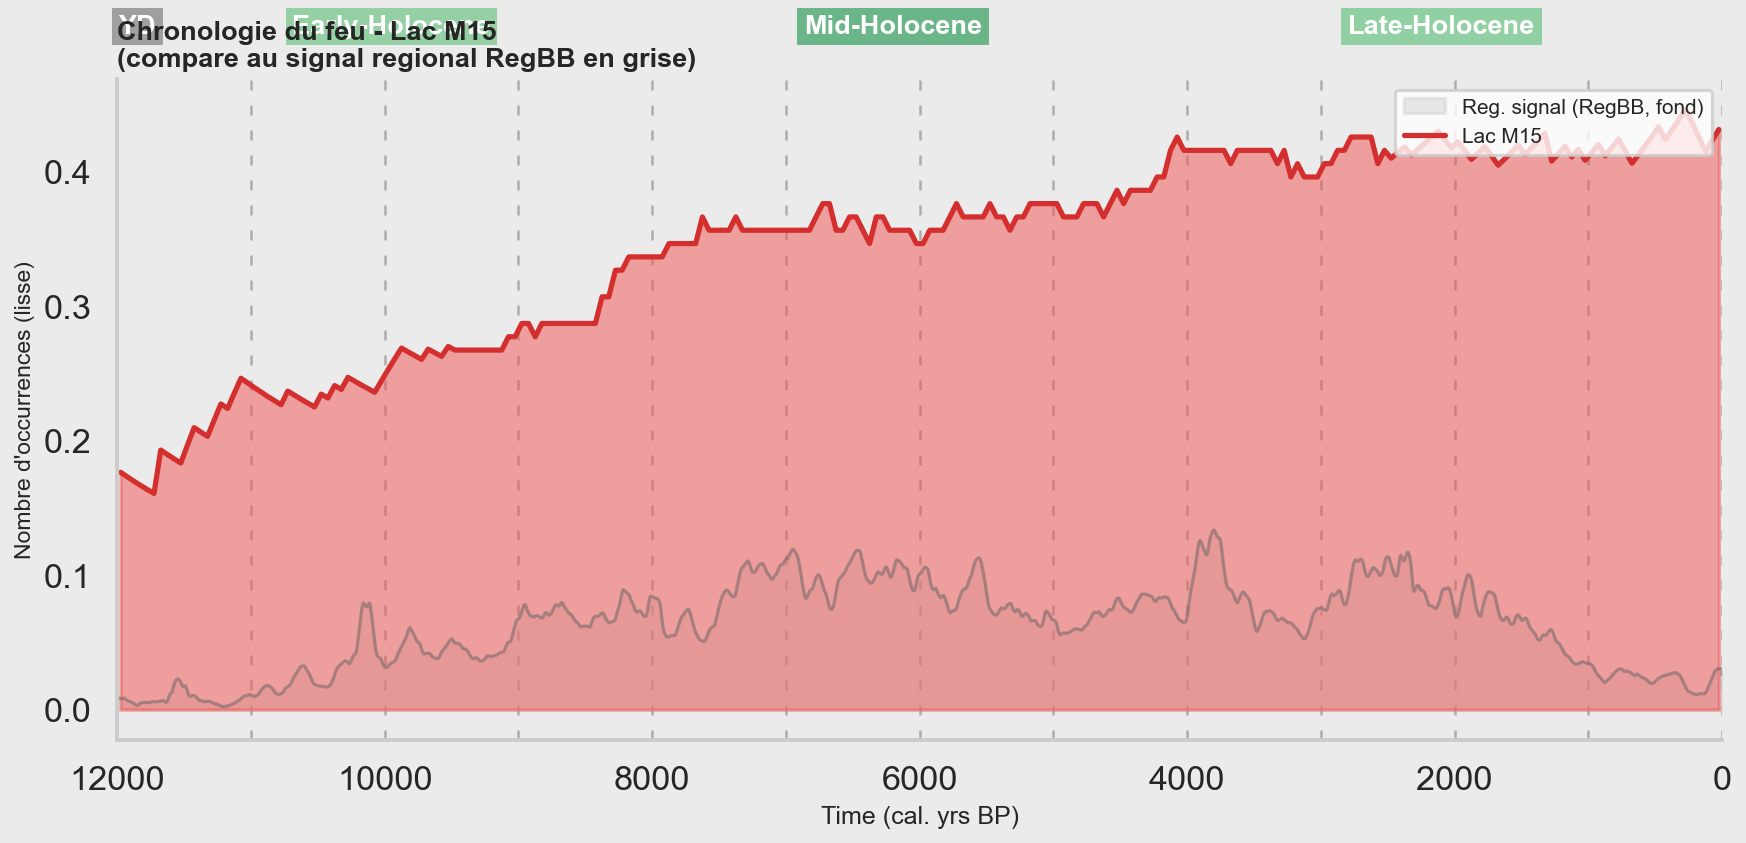
\includegraphics[width=0.85\linewidth]{fig_lac_M15_chronologie.png}
\vspace{-0.2cm}
\end{frame}

\begin{frame}{M15: traits majeurs et role regional}
\small
\begin{itemize}
  \item \alert{Pics marques}: 
  \begin{itemize}
    \item 2--3 ka: 10 ev. (maximum absolu).
    \item 4--5 ka: 8 ev. (coherent optimum moyen).
    \item 7--8 ka: 9 ev. (pic secondaire).
  \end{itemize}
  
  \item \alert{Activite tres basse}: Avant 11 ka et apres 1 ka. Signifiance chronologique.
  
  \item \alert{Superposition chronographique}: Pics M15 alignes sur RegBB regional 4--9 ka. Tres haute correlation.
  
  \item \alert{Role dans signal regional}: M15 \textit{pilote une part majeure} de la dynamique regionale observee. C'est le \textbf{site clef} de cette analyse.
\end{itemize}

\textbf{Conclusion M15:} Enregistrement de haute qualite, bien synchronise au signal moyen regional.
\end{frame}

\begin{frame}{Lac O15 (intermediaire, 67 evenements)}
  \centering
  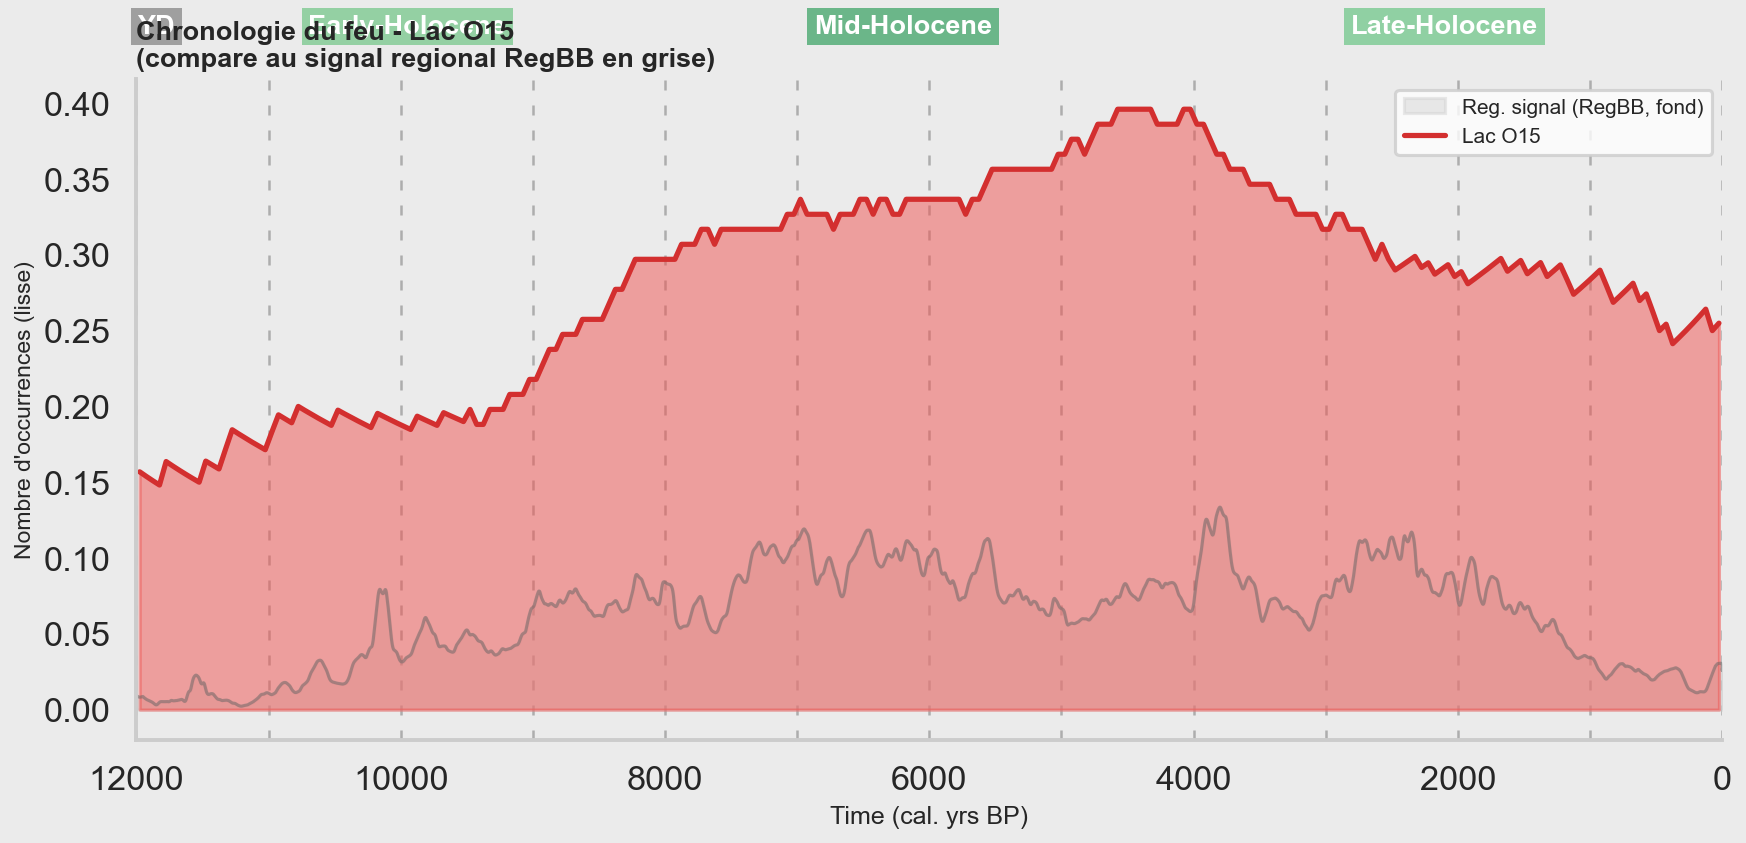
\includegraphics[width=0.85\linewidth]{fig_lac_O15_chronologie.png}
\vspace{-0.2cm}
\end{frame}

\begin{frame}{O15: traits majeurs et role regional}
\small
\begin{itemize}
  \item \alert{Pic majeur} @ 5--6 ka: 10 evenements. Synchrone au pic RegBB regional inter-annuel.
  
  \item \alert{Distribution temporelle}: Moins concentree que M15 mais remarquablement reguliere (6--8 ev./tranche, 1--10 ka).
  
  \item \alert{Baisse nette apres 11 ka et avant 1 ka}: Consistent avec region.
  
  \item \alert{Role}: Soutien directionnel de l'episode moyen-Holocene. Competence identique a O14 et O16.
\end{itemize}

\textbf{Conclusion O15:} Confirmateur du signal regional haute-frequence (4--8 ka), no specific deviations.
\end{frame}

\begin{frame}{Lac O14 (intermediaire, 67 evenements)}
  \centering
  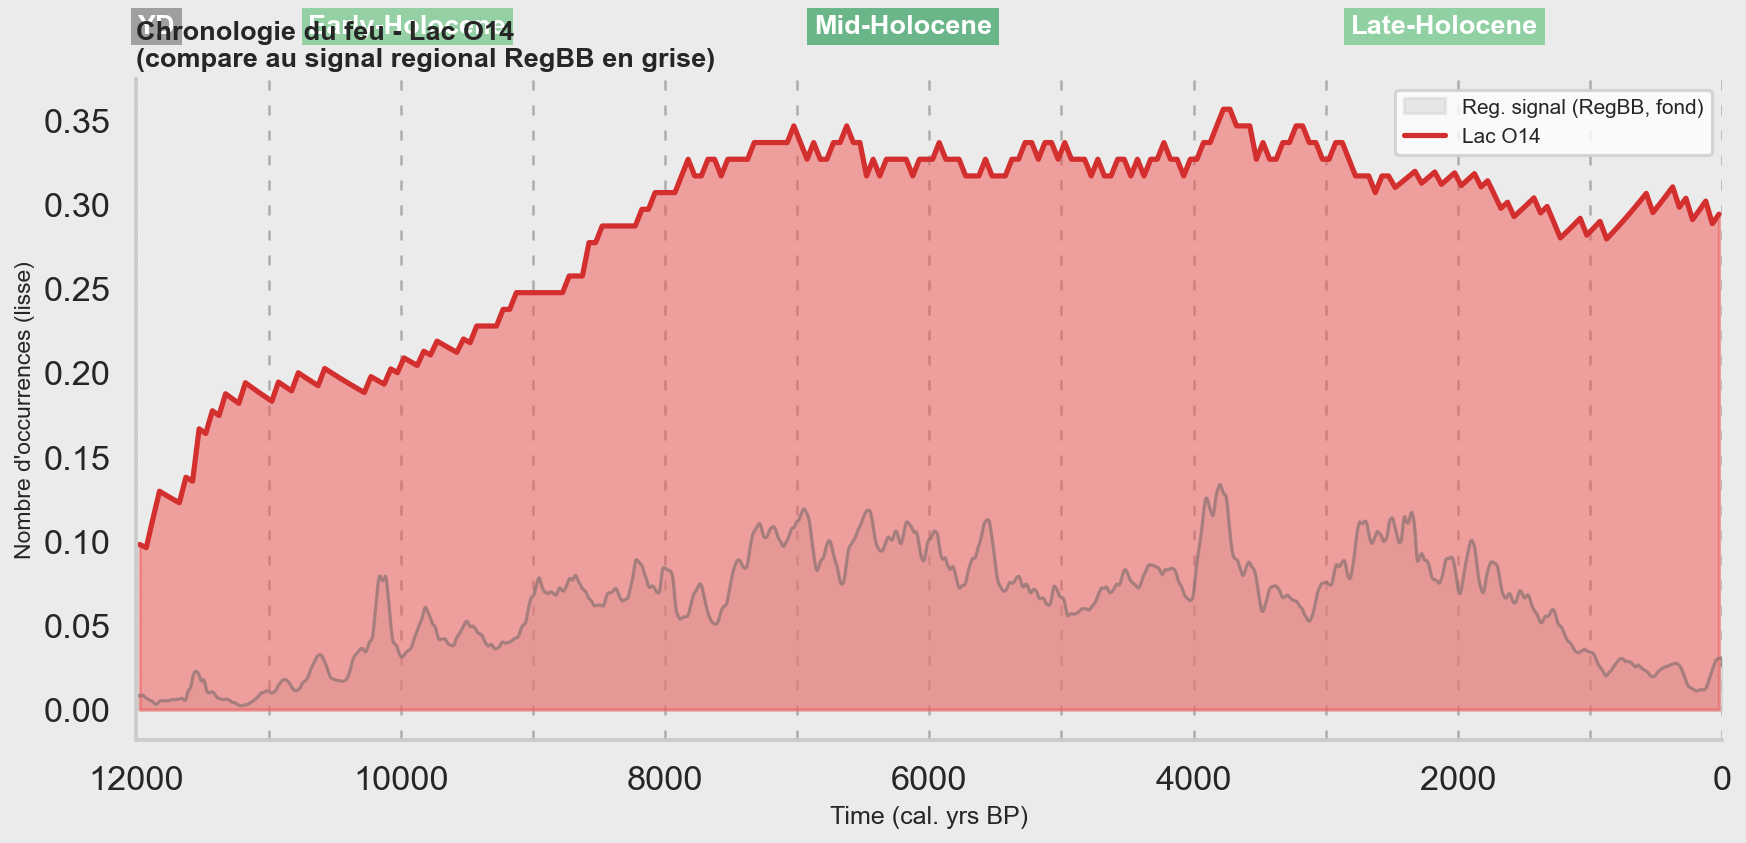
\includegraphics[width=0.85\linewidth]{fig_lac_O14_chronologie.png}
\vspace{-0.2cm}
\end{frame}

\begin{frame}{O14: uniformite remarquable}
\small
\begin{itemize}
  \item \alert{Profil exceptionnellement uniforme} 2--10 ka: 6--8 evenements par tranche de 1000 ans.
  
  \item \alert{Pas de pic marque}: Contraste absolu avec M15 (pics abruptes) et O15 (pic unique).
  
  \item \alert{Declin progressif}: Apres 10 ka, puis quasi-zero apres 1 ka.
  
  \item \alert{Interpretation}: O14 fournit un \"bruit de fond\" fiable, contribueur constant au signal regional \textbf{sans episodes locaux forts}.
\end{itemize}

\textbf{Conclusion O14:} Stabilisateur-clef du signal regional. Importance: continuite plutôt qu'amplitude.
\end{frame}

\begin{frame}{Lac O16 (double-pic, 68 evenements)}
  \centering
  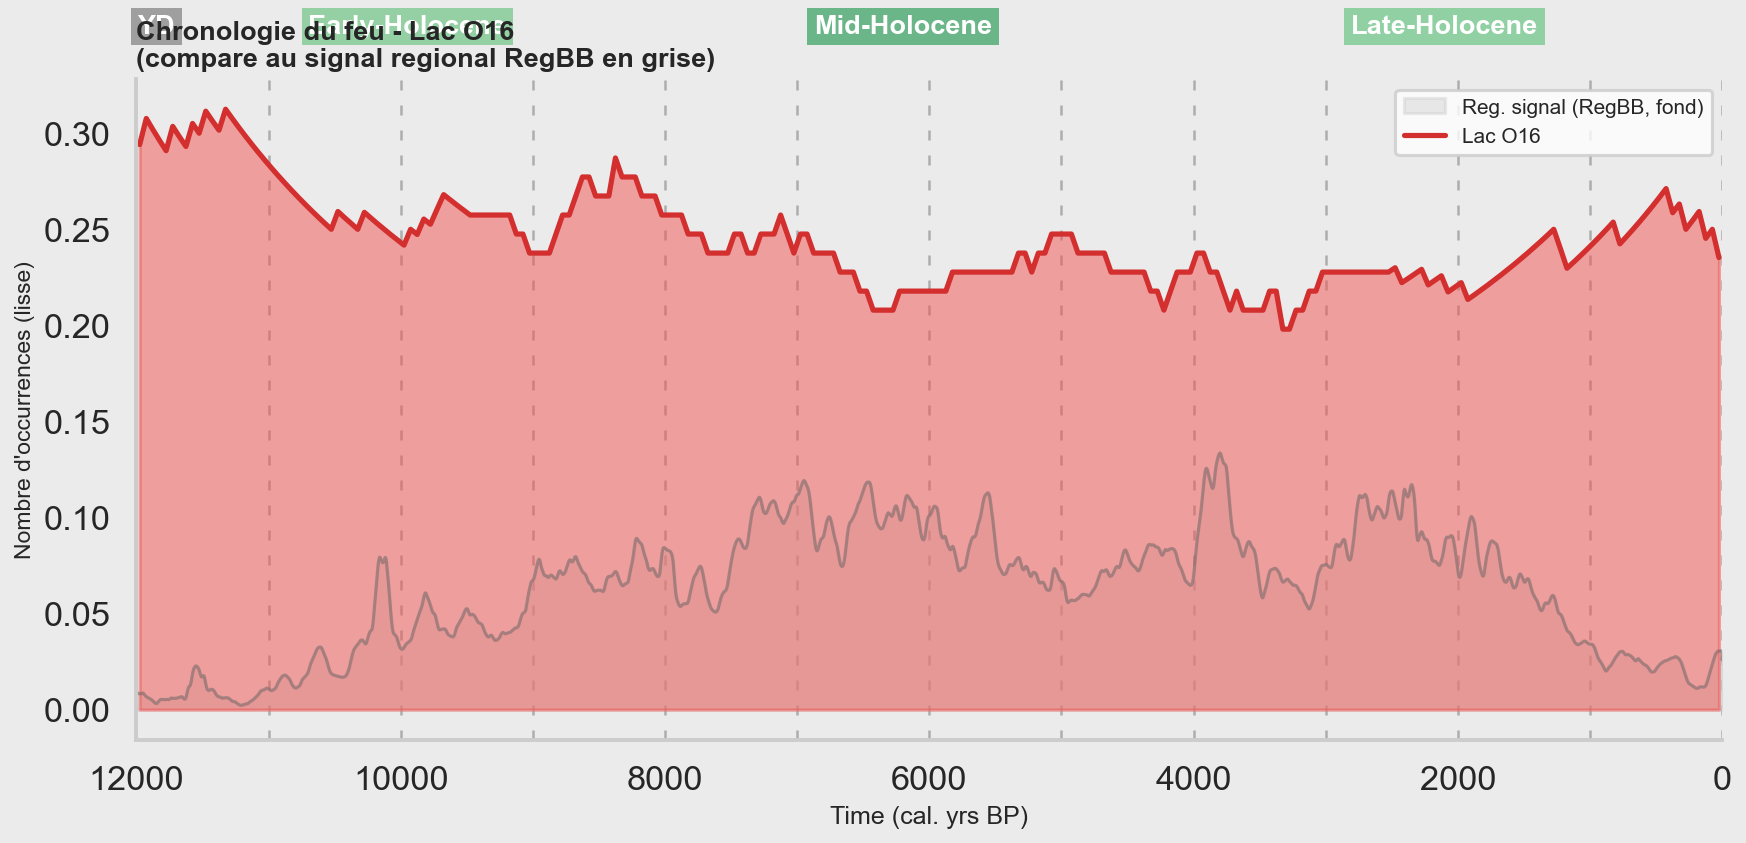
\includegraphics[width=0.85\linewidth]{fig_lac_O16_chronologie.png}
\vspace{-0.2cm}
\end{frame}

\begin{frame}{O16: desynchronisation partielle}
\small
\begin{itemize}
  \item \alert{Deux phases distinctes}:
  \begin{itemize}
    \item \textit{Phase 1}: 6--9 ka, activite forte (8 ev./tranche), pics ~6--7 ka et 9--10 ka.
    \item \textit{Phase 2}: Apres 5 ka, chute drastique (quasi-zero 0--5 ka). Desynchronisation nette.
  \end{itemize}
  
  \item \alert{Interpretation}: O16 sort partiellement du regime regional apres 5 ka. Possibles causes: changement local vegetation, modification hydrologie, ou artefact preservation.
  
  \item \alert{Robustesse signal}: Malgre cette heterogeneite, O16 ne domine pas le signal regional ($\approx 23\%$), donc \textbf{n'invalide pas conclusion}.
\end{itemize}

\textbf{Conclusion O16:} Exemple d'\alert{heterogeneite spatiale locale} --- souligne importance approche multi-lac.
\end{frame}

\begin{frame}{Lac O6 (lisse, 63 evenements)}
  \centering
  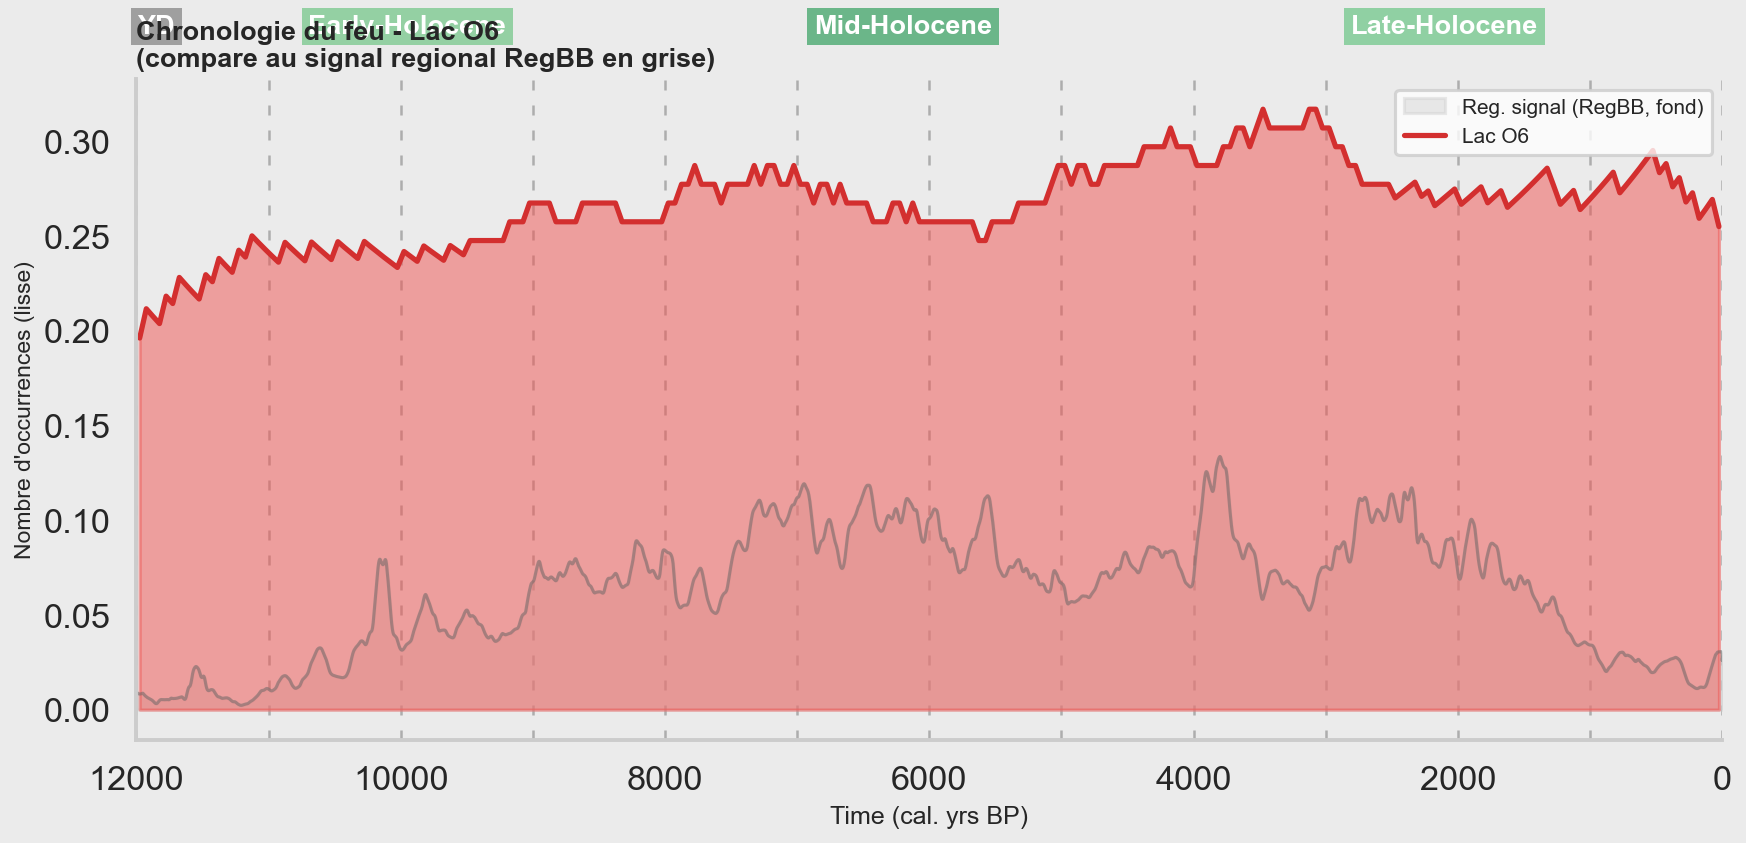
\includegraphics[width=0.85\linewidth]{fig_lac_O6_chronologie.png}
\vspace{-0.2cm}
\end{frame}

\begin{frame}{O6: profil regulier sans extrema}
\small
\begin{itemize}
  \item \alert{Remarquable lissage}: Profil quasi-identique a O14 (6--8 ev./tranche 1--10 ka).
  
  \item \alert{Pas d'extrema prononces}: Aucun pic dominant. Distribution difuse.
  
  \item \alert{Contribution constante}: Apport regulier au signal regional sans signatures markantes.
  
  \item \alert{Role}: Validateur de constance temporelle. Peu de surprises, haute fidelite relative.
\end{itemize}

\textbf{Conclusion O6:} Site de reference pour "regime normal" stationnaire.
\end{frame}

\begin{frame}{Lac M14 (marginal, 29 evenements)}
  \centering
  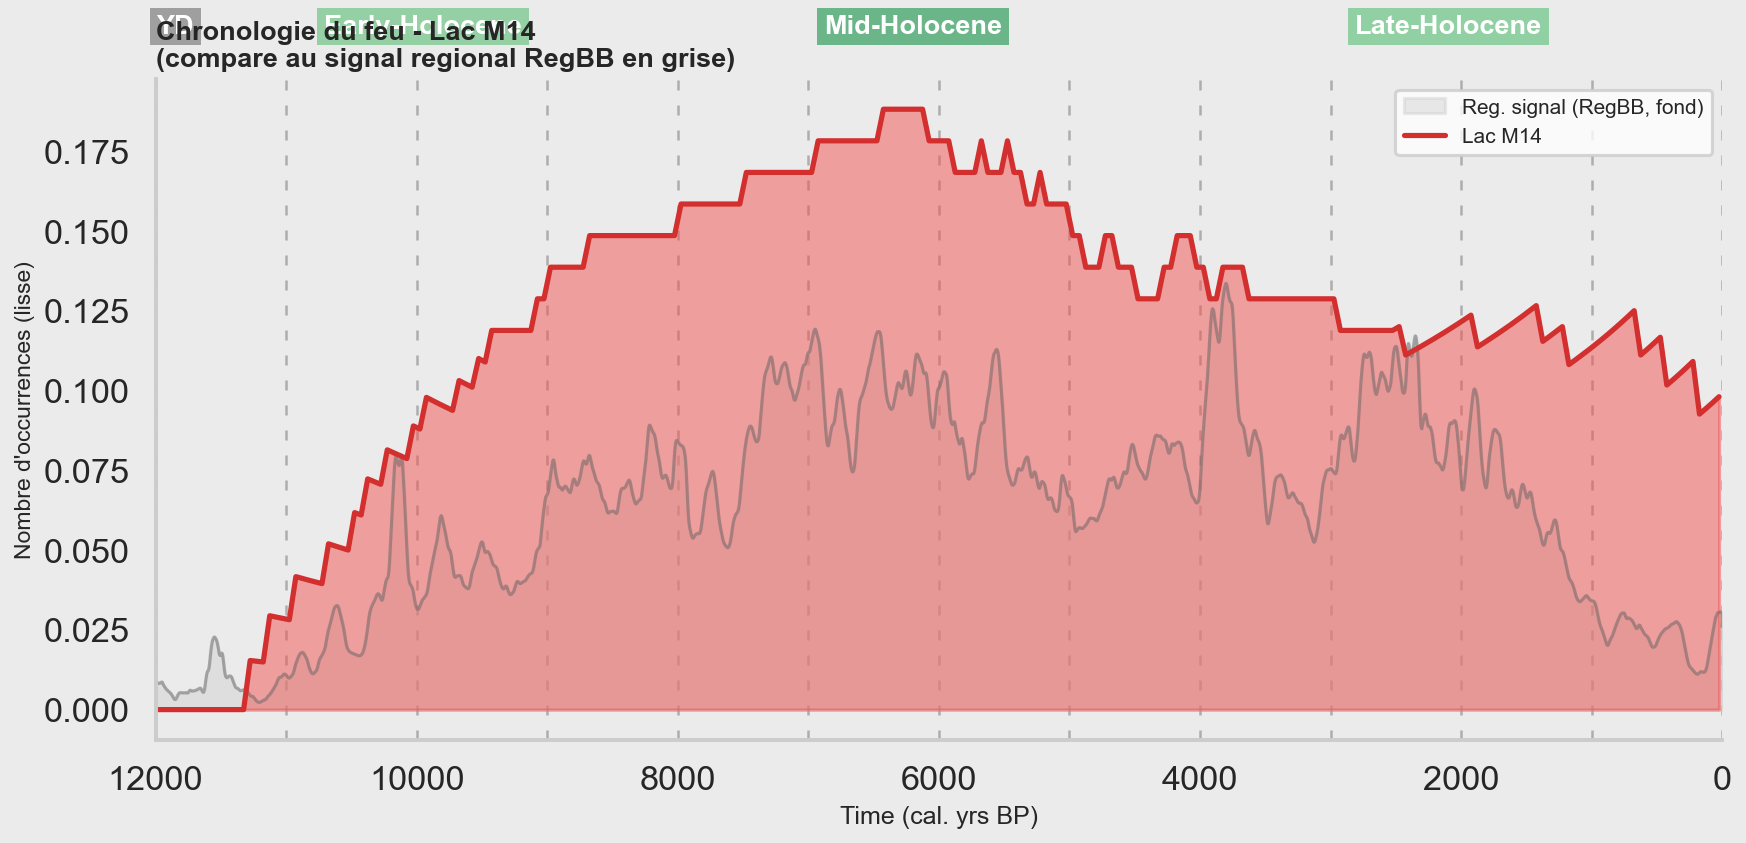
\includegraphics[width=0.85\linewidth]{fig_lac_M14_chronologie.png}
\vspace{-0.2cm}
\end{frame}

\begin{frame}{M14: marginalite persistante}
\small
\begin{itemize}
  \item \alert{Tres peu d'evenements apres 9--10 ka}: Distribution tres concentree debut.
  
  \item \alert{Apport total faible}: 29 events seulement (~10\% du total 297).
  
  \item \alert{Interpretations possibles}:
  \begin{itemize}
    \item Limitation archivage paleobotanique (compaction, migration pollen).
    \item Site specifique moins favorable a capture events.
    \item Signal reel: moins de feu apres 9 ka (+coherent regionale).
  \end{itemize}
  
  \item \alert{Role dans analyse}: Supplementaire mais \textbf{non-critique}. Can be excluded sans impact robustesse conclusion.
\end{itemize}

\textbf{Conclusion M14:} Enregistrement fragmentaire, marginal, mais presente.
\end{frame}

\section{5. Discussion et conclusions}

\begin{frame}{Signal regional vs heterogeneite locale: synthese}
\textbf{Robustesse du signal regional:}
\begin{itemize}
  \item 5--6 lacs simultanement actifs (phase 4--8 ka). Consensus spatial fort.
  
  \item Hierarchie claire: M15 + O15 pilotent les pics (~50\% poids ensemble), mais sans monopole.
  
  \item Persistance malgre O16 desynchronise, M14 marginal \textbf{renforce confiance} (robustesse statistique).
\end{itemize}

\textbf{Heterogeneite observee:}
\begin{itemize}
  \item O16: sorties regime apres 5 ka. Exemple variabilite locale reelle.
  
  \item M14: marginalite chronique. Peut traduire vraie heterogeneite ou artefact.
\end{itemize}

\textbf{Impact global:} Approche multi-lac necessaire et justifiee. Signal regional \textbf{non coincidence}: reflection vraie dynamique regionale shared.
\end{frame}

\begin{frame}{Conclusions principales}
\begin{enumerate}
  \item \textbf{Non-linearite} du regime de feu holocene boreal confirmee.
  \begin{itemize}
    \item Pas extrapolation lineaire extremites.
    \item Saut abrupt 10--8 ka vers optimum.
  \end{itemize}
  
  \item \textbf{Optimum d'activite} (4--8 ka BP) identifie \textbf{avec precision}:
  \begin{itemize}
    \item RegBB: 0.08--0.12 mm² cm$^{-1}$ yr$^{-1}$ (2x initial).
    \item RegFRI: 150--200 ans (2.5x reduction intervalle).
    \item RegFS: 0.70--0.77 (tailles soutenues).
  \end{itemize}
  
  \item \textbf{Robustesse multi-lac} documentee: M15+O15+O14+O16+O6 coherence vs M14 marginal.
  
  \item \textbf{Variabilite intra-regionale} reelle mais secondaire: heterogeneite O16 apres 5 ka, marginalite M14. Signals not erased.
  
  \item \textbf{Enjeu paleoclimatique}: Regime boreal clairement sensible aux changements climatiques rapides (optimum thermique moyen-Holocene $\sim$ 9--5 ka).
\end{enumerate}
\end{frame}

\begin{frame}{Implications et futures perspectives}
\begin{itemize}
  \item Corroborez RegBB/RegFRI/RegFS avec proxies climatiques (temp, precip, insolation).
  
  \item Analyse spectrale: frequences, periodicites, cycles.
  
  \item Modeles feedback feu-climat-vegetation: peut-on expliquer l'optimum moyen-Holocene?
  
  \item Extension spatiale (regionale, continentale): patterns comparees autres forets.
  
  \item Implications Anthropocene: quel regime attendu sous emission futures?
\end{itemize}
\end{frame}

\begin{frame}{Annexe: metodologie en detail}
\small
\textbf{Pipeline 5-etapes:}
\begin{enumerate}
  \item \textbf{Nettoyage}: Import CSV, conversion numerique, suppression NaN, fusion sur ages.
  
  \item \textbf{Metriques regionaux}: Calcul RegBB (Mean\_BB), RegFRI (1/Mean\_FF), RegFS (Mean\_FS) + IC 90\% via Infe/Supe.
  
  \item \textbf{Restriction + lissage}: Fenetre 0--12000 cal BP, lissage centre rolling-mean w=101 points.
  
  \item \textbf{Per-lac}: Histogrammes (bins 50 ans puis 500/1000 ans), lissage equiv., heatmaps, timelines.
  
  \item \textbf{Outputs}: PNG RGB DPI=150 pour figures, LaTeX Beamer + PDF pour presentation.
\end{enumerate}

\textbf{Stack technique:} Python 3.x (pandas, numpy, matplotlib, seaborn, scipy).
\end{frame}

\begin{frame}
\centering
\Huge \alert{Merci}
\vspace{0.5cm}

\Large
Questions \& Discussion
\end{frame}

\end{document}
